\documentclass[aspectratio=1610,10pt]{beamer}
\usepackage[T1]{fontenc}
\usepackage[utf8]{vietnam}
\usepackage{amsmath}
\usefonttheme[onlymath]{serif}
\usepackage{tikz}
\usepackage[most]{tcolorbox}
\usepackage{listingsutf8}
\usepackage{comment}
\usepackage{tabularx}
\usepackage{mathtools}
\usepackage{algpseudocode}
\usepackage{xcolor}
\setbeamertemplate{caption}[numbered]
\usepackage{makecell}
\usepackage{fnpct}
\usepackage{multirow}
\usepackage{bbm}
\usepackage{pgfpages}
\usepackage{handoutWithNotes}
\usepackage{xcolor}
\usepackage{calc}
\usepackage{changepage}




% Bỏ thanh mờ mờ góc phải
\setbeamertemplate{navigation symbols}{}


\setbeamercolor{section in head/foot}{bg=cyan!5, fg=cyan!50}
\setbeamercolor{author in head/foot}{bg=cyan!5, fg=black}

\setbeamerfont{section in head/foot}{size=\small}
\setbeamerfont{author in head/foot}{size=\small}

% \setbeamertemplate{footline}{
%   \begin{beamercolorbox}[ht=3ex,dp=1.5ex,right]{author in head/foot}
%     \insertframenumber{} / \inserttotalframenumber\hspace*{2ex}
%   \end{beamercolorbox}
% }

% \setbeamertemplate{headline}{%
%   \begin{beamercolorbox}[wd=\paperwidth,ht=5ex,dp=2.5ex]{section in head/foot}
%     \hspace{5 ex}
%      \insertsectionhead
%     \ifx\insertsubsectionhead\empty
%       % Không có subsection, không hiển thị dấu gạch ngang
%     \else
%       % Có subsection, hiển thị dấu gạch ngang và tên của subsection
%       \,---\,\insertsubsectionhead
%     \fi
%   \end{beamercolorbox}%
%   \vspace{5 pt}
% }

\setbeamertemplate{footline}{
    \begin{beamercolorbox}[ht=5ex,dp=3ex,right]{author in head/foot} % Tăng kích thước box
        \usebeamerfont{author in head/foot}\insertframenumber{} / \inserttotalframenumber\hspace*{2ex}
    \end{beamercolorbox}
}

\setbeamertemplate{headline}{
    \begin{beamercolorbox}[wd=\paperwidth,ht=6ex,dp=3.5ex]{section in head/foot} % Tăng kích thước box
        \usebeamerfont{section in head/foot}\hspace{1 ex}
        \insertsectionhead
        \ifx\insertsubsectionhead\empty
            % Không có subsection, không hiển thị dấu gạch ngang
        \else
            % Có subsection, hiển thị dấu gạch ngang và tên của subsection
            \,---\,\insertsubsectionhead
        \fi
    \end{beamercolorbox}%
}


\everymath{\displaystyle}


\setbeamerfont{title}{size=\fontsize{26}{12}}

% Tạo màu cho các block
\setbeamercolor{block title example}{fg=white, bg=teal!80!}
\setbeamercolor{block body example}{ bg=teal!20}
\setbeamercolor{block title alerted}{fg=white, bg=orange}
\setbeamercolor{block body alerted}{ bg=orange!25}
\setbeamercolor{block title}{bg=cyan, fg=white}
\setbeamercolor{block body}{bg=cyan!10}

% Dấu tròn trước item
\setbeamertemplate{itemize item}{\textbullet}


% Tên nè
\title{Tiny Shell}
\subtitle{
    \Large Tương tác với hệ điều hành thông qua giao diện dòng lệnh\\
    \vspace{5 pt}\small\textbf{Học phần:} IT3070 - Nguyên lý Hệ điều hành\\ \small\textbf{Giảng viên hướng dẫn:} TS. Phạm Đăng Hải}
\author{N.~V.~T.~Kiệt \inst{1,2}, B.~Q~Phong \inst{1,2}, L.~T.~Khang \inst{1}, N.~T.Tuyển \inst{1}}


\institute %
{
    \inst{1}%
    Chương trình tài năng - Khoa học máy tính K67\\
    Trường Công nghệ Thông tin và Truyền thông
    \and
    \inst{2}%
    Phòng thí nghiệm Mô hình hóa, Mô phỏng và Tối ưu hóa\\
    Trung tâm nghiên cứu quốc tế về Trí tuệ nhân tạo, BKAI

}
\date{\today}

% \setbeamertemplate{frametitle}{
% % Bọc tcolorbox bằng hbox để giới hạn chiều rộng theo nội dung
%       \begin{tcolorbox}[
%         colback=cyan!10,
%         colframe=white, % Màu viền của hộp
%         boxrule=0mm, % Độ dày của viền, đặt là 0 nếu không muốn viền
%         arc=3mm, % Độ cong của góc Tự động làm cho các góc ngoài cong theo arc được đặt
%         boxsep=1mm, % Khoảng cách giữa viền và nội dung trong hộp
%         left=3mm, right=3mm, top=1mm, bottom=1mm % Padding bên trong hộp
%       ]
%         \insertframetitle % Chèn tiêu đề slide
%       \end{tcolorbox}

% }
\newlength{\customwidth}

% \setbeamertemplate{frametitle}{
%     % Xác định chiều rộng của tiêu đề để chỉ định chiều rộng của tcolorbox
%     \settowidth{\customwidth}{\insertframetitle\hspace{6mm}}

%     \begin{tcolorbox}[
%         colback=orange!10,
%         colframe=white,
%         boxrule=0mm, % Độ dày của viền
%         arc=3mm, % Độ cong của góc
%         auto outer arc,
%         boxsep=1mm,
%         left=-1mm, right=2mm, top=0mm, bottom=1mm,
%         width=\customwidth % Đặt chiều rộng của tcolorbox bằng với chiều rộng của tiêu đề
%     ]
%         \color{orange}\insertframetitle
%     \end{tcolorbox}
% }

\setbeamertemplate{frametitle}{
    \settowidth{\customwidth}{\insertframetitle\hspace{6mm}}
    \begin{tcolorbox}[
            enhanced,
            colback=orange!10,
            colframe=white,
            boxrule=0mm,
            arc=3mm,
            auto outer arc,
            boxsep=1mm,
            left=0mm, right=1mm, top=5mm, bottom=1mm,
            width=\customwidth, % Đặt chiều rộng của tcolorbox bằng với chiều rộng giấy
            enlarge left by=-3mm, % Dịch chuyển toàn bộ tcolorbox sang trái 3mm
            overlay={
                    \node[anchor=west] at ([xshift=1mm]frame.west) {\color{orange}\insertframetitle};
                }
        ]
    \end{tcolorbox}
}



% Định nghĩa macro
\newcommand{\orange}[1]{\textbf{\textcolor{orange}{#1}}}
\newcommand{\cyan}[1]{\textbf{\textcolor{cyan}{#1}}}
\newcommand{\red}[1]{\textcolor{red}{\texttt{#1}}}

\newcommand{\mc}[1]{\ensuremath{\mathcal{#1}}}
\newcommand{\mb}[1]{\ensuremath{\mathbb{#1}}}

\newcommand{\br}[1]{\ensuremath{\left( #1 \right)}}
\newcommand{\brr}[1]{\ensuremath{\left[ #1 \right]}}
\newcommand{\brrr}[1]{\ensuremath{\left\{ #1 \right\}}}
\newcommand{\norm}[1]{\ensuremath{\lVert #1 \rVert_2}}

\newcommand{\vs}{\vspace{5pt}}
\newcommand{\rnn}[2]{\ensuremath{\mathbb{R}^{{#1}\times{#2}}}}
\newcommand{\rnnn}[3]{\ensuremath{\mathbb{R}^{{#1}\times{#2}\times{#3}}}}

\renewcommand{\v}[1]{\mathbf{#1}}

\renewcommand{\t}[1]{\texttt{#1}}

% \usepackage{handoutWithNotes}
% \pgfpagesuselayout{1 on 1 with notes}[a4paper,border shrink=5mm]

\AtBeginSection[]{
\begin{frame}
\tableofcontents[currentsection]
\end{frame}
}

\begin{document}

\begin{frame}
\titlepage
\end{frame}

\begin{frame}{Mục lục}
\tableofcontents[hideallsubsections]
\end{frame}

%%%%%%%%%%%%%%%%%%%%%%%%%%%%%%%%%%%%%%%%%%%%%%%%%%%%%

\section{Giới thiệu chung}

\subsection{Khái niệm}

\begin{frame}{Giao diện dòng lệnh}
\begin{itemize}
    \it em \cyan{Giao diện dòng lệnh} (Command Line Interface - CLI) là một phương thức tương tác giữa người dùng và hệ thống máy tính. \\
    $\to$ Người dùng nhập các lệnh dưới \orange{dạng văn bản} và nhận phản hồi dưới dạng văn bản.\\
    $\to$ \underline{Yêu cầu} người dùng có kiến thức về các lệnh và cú pháp.
    \item Chương trình xử lý giao diện dòng lệnh được gọi là Trình thông dịch dòng lệnh (command-line interpreter), Trình xử lý dòng lệnh (command-line processor), hay Shell.
\end{itemize}
\end{frame}

\begin{frame}{Lời gọi hệ thống}
    \begin{itemize}
        \item \cyan{Lời gọi hệ thống} (system call) là một giao diện mà chương trình ứng dụng (user application) sử dụng để yêu cầu các dịch vụ từ hệ điều hành.
        \item Lời gọi hệ thống thường được gọi thông qua các hàm thư viện trong ngôn ngữ lập trình.\\
        \vspace{10 pt}
        \orange{Ví dụ:}
        \begin{itemize}
            \item Trên Unix/Linux: \t{open()}, \t{wait()}, \t{mmap()}, \t{socket()},...
            \item Trên Windows: \t{CreateFile()}, \t{WaitForSingleObject()}, \t{VirtualAlloc()},...
        \end{itemize}
        \item Trên Windows, các lời gọi hệ thống được cung cấp thông qua các API của Windows, chủ yếu từ Windows API (WinAPI). Các lời gọi hệ thống trên Windows thường phức tạp hơn và bao gồm nhiều chức năng bổ sung để tương thích với kiến trúc của Windows. 
    \end{itemize}
\end{frame}

\subsection{Windows API}
\begin{frame}{Windows API}
\begin{itemize}
    \item \cyan{Windows API} là một tập hợp các giao diện lập trình ứng dụng được Microsoft cung cấp, cho phép các phần mềm tương tác với hệ điều hành Windows.
    \item \underline{Chức năng:} WinAPI cung cấp các chức năng cần thiết để quản lý tệp, tiến trình, bộ nhớ, giao tiếp mạng và nhiều hơn nữa.
\end{itemize}

\end{frame}

\begin{frame}
\begin{table}[h]
\centering
\begin{tabular}{|>{\raggedright}m{3cm}|>{\raggedright\arraybackslash}m{4.5cm}|>{\raggedright\arraybackslash}m{4.5cm}|}
\hline
\textbf{Tính năng}             & \textbf{Windows (WinAPI)}                                    & \textbf{Unix/Linux}                                       \\ \hline
\textbf{Quản lý tệp}       & \texttt{CreateFile}, \texttt{ReadFile}, \texttt{WriteFile}, \texttt{CloseHandle}        & \texttt{open}, \texttt{read}, \texttt{write}, \texttt{close}                         \\ \hline
\textbf{Quản lý tiến trình} & \texttt{CreateProcess}, \texttt{WaitForSingleObject}, \texttt{TerminateProcess} & \texttt{fork}, \texttt{exec}, \texttt{wait}, \texttt{kill}                           \\ \hline
\textbf{Quản lý bộ nhớ}    & \texttt{VirtualAlloc}, \texttt{VirtualFree}                           & \texttt{mmap}, \texttt{munmap}, \texttt{brk}                                \\ \hline
\textbf{Giao tiếp mạng}    & Winsock: \texttt{socket}, \texttt{bind}, \texttt{listen}, \texttt{accept}, \texttt{connect}      & BSD Sockets: \texttt{socket}, \texttt{bind}, \texttt{listen}, \texttt{accept}, \texttt{connect} \\ \hline
\textbf{Tính mở rộng}      & Nhiều tùy chọn và tham số                           & Thường đơn giản, ít tùy chọn hơn                 \\ \hline
\textbf{Tài liệu hỗ trợ}   & Phong phú, chi tiết                                 & Tài liệu tốt nhưng không phong phú bằng Windows  \\ \hline
\end{tabular}
\caption{So sánh lời gọi hệ thống giữa Windows và Unix/Linux}
\end{table}
\end{frame}

\begin{frame}
\begin{itemize}
    \item Để biên dịch các chương trình sử dụng Windows API, bạn cần đảm bảo rằng trình biên dịch của bạn được cấu hình đúng để liên kết với các thư viện cần thiết. 
    \item Để sử dụng các hàm Windows API, bạn cần bao gồm tệp tiêu đề \texttt{<windows.h>} trong mã nguồn C++ của bạn. Đây là tệp tiêu đề chính chứa các khai báo cho hầu hết các hàm Windows API.
\end{itemize}
\end{frame}

\subsection{Shell}

\begin{frame}{Shell trong Windows}
Shell trong Windows là một giao diện cho phép người dùng tương tác với hệ điều hành và quản lý tài nguyên máy tính.
\vspace{5 pt}
Các loại Shell trong Windows:
\begin{itemize}
    \item \cyan{Windows Shell (Graphical Shell):} giao diện đồ họa người dùng (GUI) chính.
    \item \orange{Command Prompt (CMD):} giao diện dòng lệnh (CLI) truyền thống.
    \item \orange{PowerShell:} công cụ dòng lệnh mạnh mẽ và một ngôn ngữ script được thiết kế cho quản trị hệ thống và tự động hóa trên Windows. 
\end{itemize}
\end{frame}

\begin{frame}
\begin{table}[h]
\centering
\begin{tabular}{|>{\raggedright}m{2cm}|>{\raggedright\arraybackslash}m{3cm}|>{\raggedright\arraybackslash}m{3.5cm}|}
\hline
\textbf{Tính năng} & \textbf{CMD} & \textbf{PowerShell} \\ \hline
\textbf{Ngôn ngữ} & Dòng lệnh cơ bản & Ngôn ngữ script mạnh mẽ dựa trên .NET \\ \hline
\textbf{Cmdlets} & Không có & Hàng ngàn cmdlets mạnh mẽ \\ \hline
\textbf{Pipeline} & Hạn chế & Mạnh mẽ và linh hoạt \\ \hline
\textbf{Scripting} & Hỗ trợ các script \texttt{.bat} đơn giản & Hỗ trợ script mạnh mẽ với \texttt{.ps1} \\ \hline
\textbf{Tích hợp .NET} & Không có & Tích hợp sâu với .NET \\ \hline
\textbf{Khả năng tự động hóa} & Hạn chế & Mạnh mẽ và linh hoạt \\ \hline
\end{tabular}
\caption{So sánh giữa CMD và PowerShell}
\end{table}
\end{frame}

\section{Tiny Shell}

\subsection{Cài đặt và triển khai}
\begin{frame}{Môi trường phát triển}
 \begin{itemize}
        \item \cyan{Ngôn ngữ lập trình:} C++ 17 hoặc lớn hơn
        \item \cyan{Trình biên dịch:} g++ (Rev3, Built by MSYS2 project) 13.2.0
        \item \cyan{Phần mềm:} IDE Visual Studio Code V1.90.0 hoặc phiên bản mới nhất
        \item \cyan{Hệ điều hành:} Windows 10 trở lên, tốt nhất nếu Windows 11
    \end{itemize}
\end{frame}

\begin{frame}{Cấu trúc mã nguồn}
\cyan{Tổ chức mã nguồn}\footnote{\orange{Mã nguồn dự án:} \href{https://github.com/HaiAu2501/Operating-System-Project}{Operating System Project}. \orange{Hướng dẫn sử dụng:} \href{https://github.com/HaiAu2501/Operating-System-Project/blob/main/README.md}{README}}: Dễ đọc, dễ quản lý, dễ sử dụng kèm hướng dẫn chi tiết.
\begin{figure}[h]
        \centering
        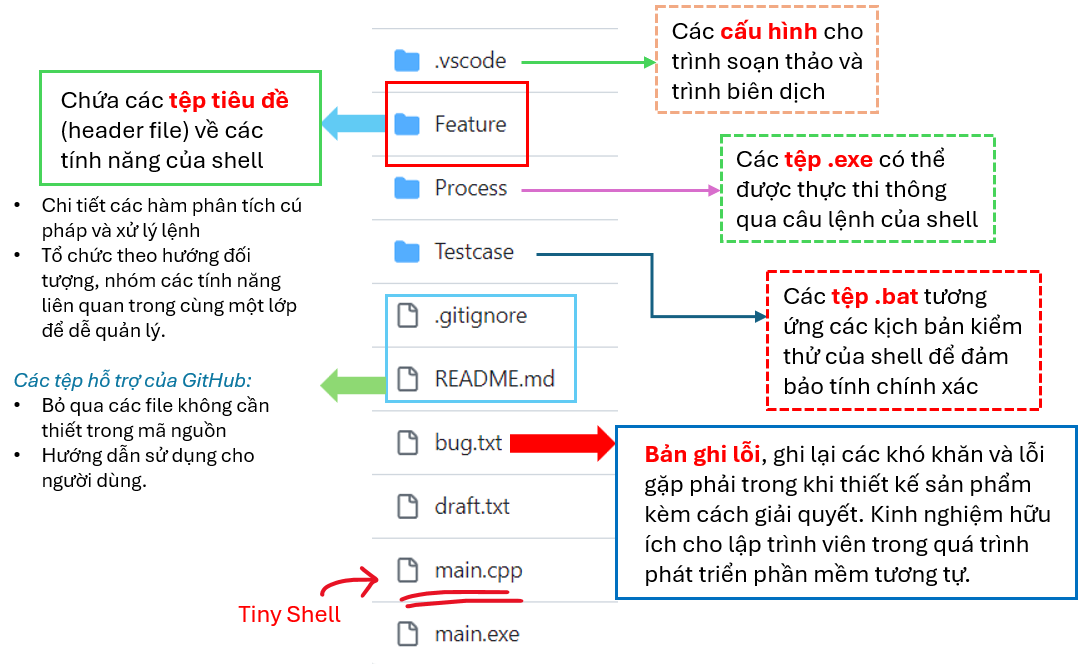
\includegraphics[width=0.65\textwidth]{images/03.png}
    \end{figure}
\end{frame}

\begin{frame}
\begin{enumerate}
    \item Sau khi biên dịch tệp \t{main.cpp} và chạy chương trình \t{main.exe} thành công, bạn có thể chính thức sử dụng Tiny Shell.
\end{enumerate}
    \begin{figure}[h]
        \centering
        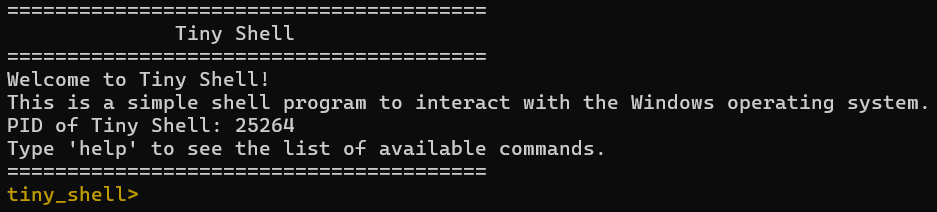
\includegraphics[width=0.9\textwidth]{images/01.png}
        \caption{Màn hình hiện lên sau khi khởi chạy Tiny Shell}
    \end{figure}
\end{frame}

\begin{frame}
\begin{enumerate}
    \setcounter{enumi}{1}
    \item Hãy bắt đầu với lệnh \t{help} để xem \orange{danh sách các lệnh} mà Tiny Shell hỗ trợ.\\
    $\to$ Nếu không rõ cú pháp lệnh, hay gõ (sai) lệnh và Tiny Shell sẽ thông báo.\\
    \vspace{10 pt}
    \orange{Ví dụ:}\\
    \begin{figure}
        \centering
        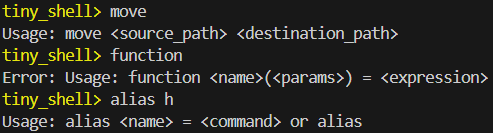
\includegraphics{images/04.png}
        \caption{Nếu nhập sai cú pháp lệnh, Tiny Shell sẽ nhắc nhở cú pháp đúng}
    \end{figure}
\end{enumerate}
\end{frame}

\begin{frame}
\begin{enumerate}
    \setcounter{enumi}{2}
    \item Tiny Shell hỗ trợ \cyan{70 lệnh cơ bản} và tổng cộng \cyan{90 cú pháp lệnh}. Trong đó:
    \begin{itemize}
        \item Quản lý tệp và thư mục: 15 lệnh.
        \item Quản lý tiến trình: 11 lệnh.
        \item Hệ thống và tiện ích: 17 lệnh.
        \item Điều hướng và giao diện: 10 lệnh.
        \item Tính toán nâng cao: 18 lệnh.
    \end{itemize}
    \item Lấy cảm hứng từ CMD và PowerShell của hệ điều hành Windows.\\
    $\to$ Tiny Shell còn có những \orange{tính năng riêng đặc biệt}, cung cấp nhiều tiện ích để người dùng dễ dàng giao tiếp với máy tính. 
\end{enumerate}
\end{frame}

\subsection{Các tính năng cơ bản}

\begin{frame}{Quản lý tệp}
Tiny Shell có thể thực hiện một số thao tác với tệp:
\begin{table}
    \centering
    \begin{tabular}{l|l}
         \cyan{Tính năng thiết yếu} & \cyan{Tính năng nâng cao} \\
         \hline
         \t{open} &  \t{check\_file} \\
         \t{move\_file} & \t{file\_size} \\
         \t{rename\_file} & \red{read\_file}: hỗ trợ đọc theo dòng \\
         \t{delete\_file} & \red{write\_file}: hỗ trợ ghi theo dòng \\
         \t{create\_file} &  \red{extension\_file}: xem phần mở rộng\\
         \t{copy\_file} & \red{list\_file}: liệt kê file với phần mở rộng \\
    \end{tabular}
    \caption{Một số câu lệnh đối với tệp}
    \label{tab:my_label}
\end{table}
\end{frame}

\begin{frame}
\begin{figure}
    \centering
    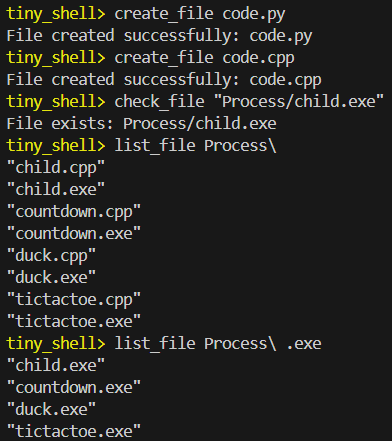
\includegraphics[width=0.4\textwidth]{images/05.png}
    \caption{Chạy các câu lệnh với kịch bản kiểm thử về file}
    \label{fig:enter-label}
\end{figure}
\end{frame}

\begin{frame}{Quản lý thư mục}
Tiny Shell có thể thực hiện một số thao tác với thư mục:
\begin{itemize}
    \item \t{create}
    \item \t{open}
    \item \t{delete}
    \item \t{copy}
    \item \t{rename}
    \item \t{move}
    \item \t{cd}
    \item \t{dir}
    \item \t{pwd}
    \item \t{list\_tree}
\end{itemize}
\end{frame}

\begin{frame}
\begin{figure}
    \centering
    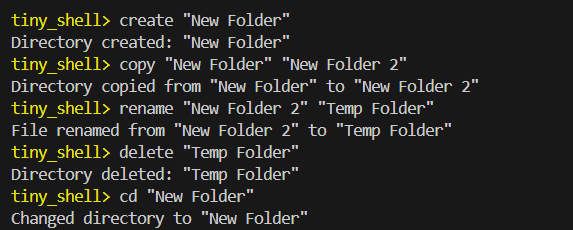
\includegraphics[width=0.75\textwidth]{images/07.png}
    \caption{Chạy các câu lệnh với kịch bản kiểm thử về thư mục}
    \label{fig:enter-label}
\end{figure}
\end{frame}

\begin{frame}{Quản lý tiến trình}
Tiny Shell chứa các câu lệnh quản lí tiến trình:
\begin{table}[h]
    \centering
    \begin{tabular}{l|l}
         \textbf{Lệnh} & \textbf{Mô tả lệnh} \\
         \hline
         \t{list\_processes} & In ra danh sách tiến trình \\
         \red{start\_foreground} & Tạo tiến trình con ở trạng thái foreground \\
         \red{start\_background} & Tạo tiến trình con ở trạng thái background \\
         \red{terminate} & Chấm dứt một tiến trình \\
         \red{suspend} & Tạm dừng một tiến trình \\
         \red{resume} & Tiếp tục một tiến trình \\
    \end{tabular}
    \caption{Một số câu lệnh đối với tiến trình}
    \label{tab:process_management}
\end{table}
\end{frame}

\begin{frame}
\begin{figure}
    \centering
    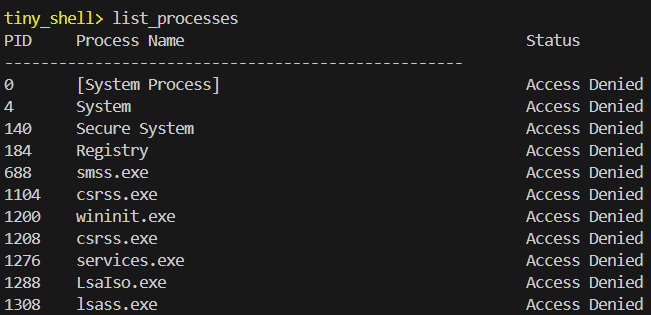
\includegraphics[width=0.9\textwidth]{images/21.png}
    \caption{Câu lệnh liệt kê tiến trình}
    \label{fig:enter-label}
\end{figure}
\end{frame}

\begin{frame}
\begin{table}[h]
    \centering
    \begin{tabular}{l|l}
         \textbf{Lệnh nâng cao} & \textbf{Mô tả lệnh} \\
         \hline
         \t{list\_children} & In ra danh sách tiến trình con \\
         \t{manage\_threads} & Quản lý luồng \\
         \t{child} & Tạo một tiến trình con đơn giản (background) \\
         \t{countdown} & Tạo một cửa sổ đếm ngược 10 giây (background) \\
         \t{duck} & Tạo một chú vịt bơi trên màn hình (foreground)\\
         \t{tictactoe} & Khởi động trò chơi Tic-Tac-Toe trên màn hình (foreground) \\
         \t{dancing} & Hiển thị một khuôn mặt nhảy múa trên màn hình (foreground) \\
         \red{after} & Lên lịch chạy câu lệnh sau một khoảng thời gian \\
    \end{tabular}
    \caption{Một số câu lệnh nâng cao đối với tiến trình}
    \label{tab:process_management}
\end{table}
Trong đó:
\begin{itemize}
    \item Nếu đang có tiến trình con chạy foreground và người dùng ấn tổ hợp phím \orange{Ctrl + C} thì tiến trình con sẽ dừng và trở về Shell chính.
    \item Nếu Shell đang chạy và người dùng ấn tổ hợp phím \orange{Ctrl + C} thì không khiến Shell dừng, thay vào đó, nó bỏ qua dòng hiện tại tạo ra dòng mới \t{tiny\_shell>}.
\end{itemize}
\end{frame}

\begin{frame}
\begin{figure}
    \centering
    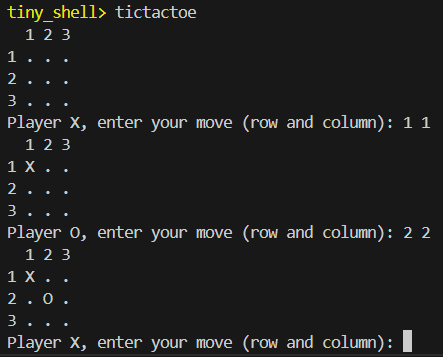
\includegraphics[width=0.6\textwidth]{images/22.png}
    \caption{Chạy Tic-Tac-Toe (foreground), có thể ấn Ctrl + C để thoát và quay lại Tiny Shell}
    \label{fig:enter-label}
\end{figure}
\end{frame}

\begin{frame}{Quản lý biến môi trường}
Tiny Shell chứa các câu lệnh quản lý đường dẫn và biến môi trường:
\begin{table}[h]
    \centering
    \begin{tabular}{l|l}
         \textbf{Lệnh} & \textbf{Mô tả lệnh} \\
         \hline
         \t{add\_path} & Thêm một đường dẫn vào PATH \\
         \t{is\_in\_path} & Kiểm tra xem một đường dẫn có nằm trong PATH hay không \\
         \t{remove\_path} & Xóa một đường dẫn khỏi PATH \\
         \red{set\_env} & Thiết lập một biến môi trường \\
         \red{unset\_env} & Hủy bỏ một biến môi trường \\
         \red{print\_env} & In giá trị của một biến môi trường cụ thể \\
         \t{list\_env} & Liệt kê tất cả các biến môi trường \\
         \t{save\_env} & Lưu các biến môi trường vào một tệp \\
         \t{load\_env} & Tải các biến môi trường từ một tệp \\
    \end{tabular}
    \caption{Một số câu lệnh đối với đường dẫn và biến môi trường}
    \label{tab:path_env_management}
\end{table}
\end{frame}

\begin{frame}
\begin{figure}
    \centering
    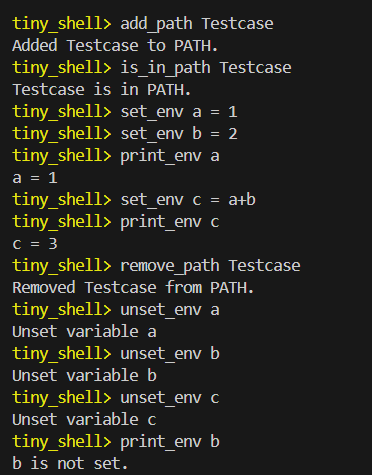
\includegraphics[width=0.4\textwidth]{images/09.png}
    \caption{Chạy các câu lệnh với kịch bản kiểm thử về đường dẫn và biến môi trường}
    \label{fig:enter-label}
\end{figure}
\end{frame}

\subsection{Các tính năng nâng cao}

\begin{frame}{Tiện ích hệ thống}
Tiny Shell có thể hiểu một số lệnh về tiện ích hệ thống:
\begin{table}[h]
    \centering
    \begin{tabular}{l|l}
         \textbf{Lệnh thiết yếu} & \textbf{Mô tả lệnh} \\
         \hline
         \t{time} & Hiển thị thời gian hiện tại \\
         \t{date} & Hiển thị ngày hiện tại \\
         \t{uptime} & Hiển thị thời gian hệ thống đã hoạt động \\
         \t{cpuinfo} & Hiển thị thông tin về CPU \\
         \t{meminfo} & Hiển thị thông tin về bộ nhớ \\
         \t{diskinfo} & Hiển thị thông tin về đĩa cứng \\
         \t{calculator} & Mở máy tính \\
    \end{tabular}
    \caption{Một số câu lệnh đối với tiện ích hệ thống}
    \label{tab:system_utilities}
\end{table}
\end{frame}

\begin{frame}
\begin{figure}
    \centering
    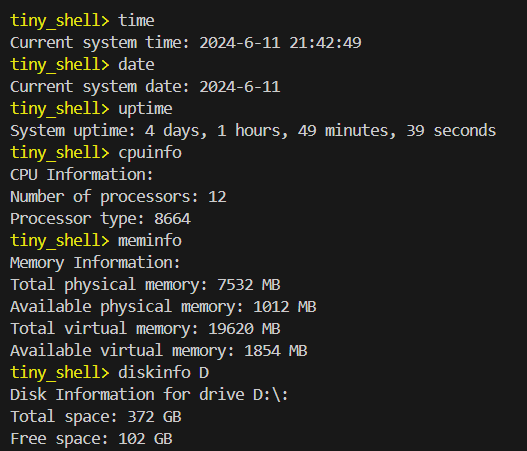
\includegraphics[width=0.6\textwidth]{images/08.png}
    \caption{Chạy các câu lệnh với kịch bản kiểm thử với các tiện ích hệ thống}
    \label{fig:enter-label}
\end{figure}
\end{frame}

\begin{frame}
\begin{table}[h]
    \centering
    \begin{tabular}{l|l}
         \textbf{Lệnh nâng cao} & \textbf{Mô tả lệnh} \\
         \hline
         \red{exit} & Thoát khỏi shell \\
         \red{help} & Hiển thị trợ giúp về các lệnh có sẵn \\
         \red{history} & Hiển thị lịch sử các lệnh đã nhập \\
         \red{clear} & Xóa màn hình hiển thị của shell \\
         \red{clear\_history} & Xóa lịch sử các lệnh đã nhập \\
         \red{change\_color} & Đổi màu chữ của shell
    \end{tabular}
    \caption{Một số câu lệnh nâng cao đối với tiện ích hệ thống}
    \label{tab:system_utilities}
\end{table}
\end{frame}

\begin{frame}
\begin{figure}
    \centering
    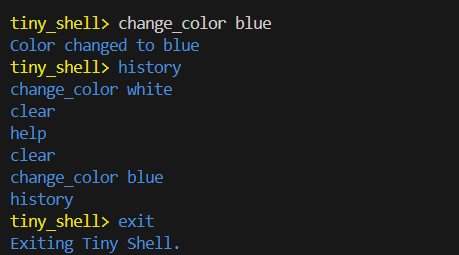
\includegraphics[width=0.6\textwidth]{images/13.png}
    \caption{Chạy một số câu lệnh nâng cao kiểm thử các tiện ích hệ thống}
    \label{fig:enter-label}
\end{figure}
\end{frame}

\begin{frame}{Thực thi kịch bản}
\begin{itemize}
    \item Thư mục Testcase\footnote{\orange{Mã nguồn dự án:} \href{https://github.com/HaiAu2501/Operating-System-Project/tree/main/Testcase}{Kịch bản kiểm thử}} chứa các kịch bản kiểm thử. Mỗi kịch bản là dãy lệnh của Tiny Shell được lưu thành một file \t{.bat}.
    \item Tiny Shell có thể thực hiện các câu lệnh được viết trong file \t{.bat}.
\end{itemize}
\begin{figure}
    \centering
    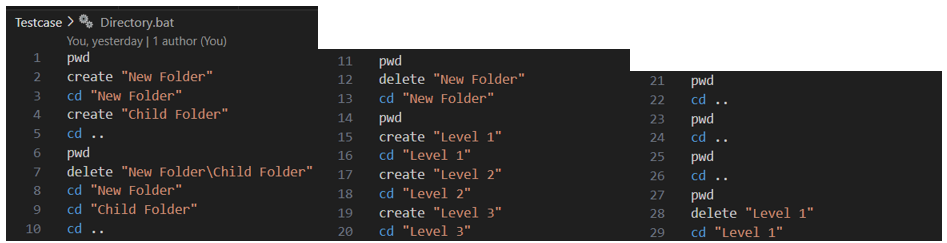
\includegraphics[width=\textwidth]{images/06.png}
    \caption{Minh họa một kịch bản kiểm tra dãy lệnh với thư mục}
    \label{fig:enter-label}
\end{figure}
\end{frame}

\begin{frame}{Tính toán nâng cao}
Tiny Shell có thể hiểu một số lệnh về tính toán và điều kiện.
\begin{table}[h]
    \centering
    \begin{tabular}{l|l}
         \textbf{Lệnh} & \textbf{Mô tả lệnh} \\
         \hline
         \red{calculate} & Tính giá trị một biểu thức \\
         \red{function} & Định nghĩa một hàm \\
         \red{evaluate} & Tính giá trị của một hàm tại giá trị cụ thể \\
                  \t{convert} & Chuyển đổi hệ cơ số \\
    \end{tabular}
    \caption{Một số lệnh đối với tính toán và điều kiện}
    \label{tab:calculation_condition}
\end{table}
\begin{itemize}
    \item Biểu thức nhập vào dưới dạng trung tố (infix), sau đó sử dụng \cyan{thuật toán Shunting Yard} chuyển biểu thức trung tố sang biểu thức hậu tố (postfix) để tính toán giá trị.
    \item Một số câu lệnh vòng lặp và điều kiện không thể hoàn thiện như ngôn ngữ lập trình.
\end{itemize}
\end{frame}

\begin{frame}
\begin{figure}
    \centering
    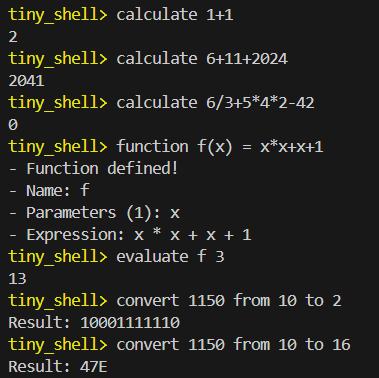
\includegraphics[width=0.5\textwidth]{images/10.png}
    \caption{Chạy các câu lệnh kiểm thử chức năng tính toán}
    \label{fig:enter-label}
\end{figure}
\end{frame}

\subsection{Các tiện ích mở rộng}

\begin{frame}{Các tiện ích mở rộng}
Shell có thể thực hiện một số tiện ích khác như:
\begin{table}[h]
    \centering
    \begin{tabular}{l|l}
         \textbf{Lệnh} & \textbf{Mô tả lệnh} \\
         \hline
         \t{alias} & Định nghĩa viết tắt của câu lệnh \\
         \t{unalias} & Hủy định nghĩa viết tắt của câu lệnh \\
         \t{bookmark} & Định nghĩa tên gọi tắt cho đường dẫn \\
        \red{loop} & Thực hiện một lệnh lặp với số vòng cụ thể \\
         \red{if else} & Thực hiện biểu thức điều kiện \\
    \end{tabular}
    \caption{Một số lệnh đối với tiện ích mở rộng}
    \label{tab:additional_commands}
\end{table}
\end{frame}

\begin{frame}
\begin{figure}
    \centering
    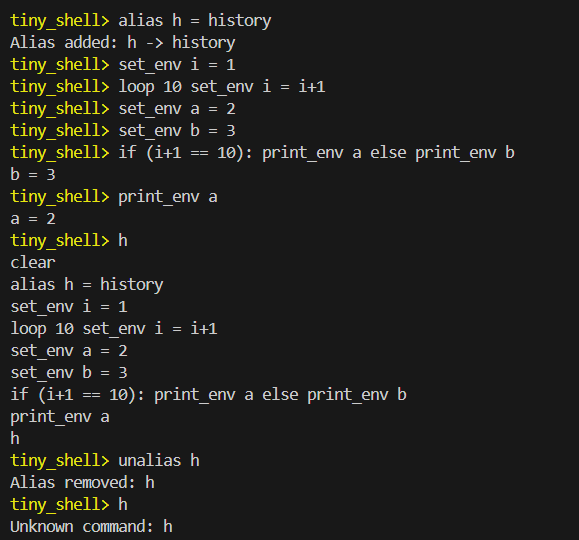
\includegraphics[width=0.55\textwidth]{images/11.png}
    \caption{Chạy các câu lệnh kiểm thử các tiện ích mở rộng}
    \label{fig:enter-label}
\end{figure}
\end{frame}

\section{Kết luận \& Thảo luận}

\subsection{Tính ứng dụng}

\begin{frame}{Ứng dụng trong học tập}
Sản phẩm \orange{Tiny Shell}, mô phỏng giao diện dòng lệnh shell để người dùng tương tác với hệ điều hành, có nhiều tính ứng dụng quan trọng và giá trị trong học tập:
\vspace{5 pt}
\begin{itemize}
    \item Hiểu sâu hơn về cách hệ điều hành quản lý và thực thi các lệnh từ người dùng, cách xử lý các tiến trình và cách giao tiếp với phần cứng.
    \item Xây dựng một shell yêu cầu hiểu biết về lập trình hệ thống, bao gồm quản lý bộ nhớ, quản lý tiến trình và xử lý tín hiệu $\to$ \cyan{củng cố kiến thức lập trình C/C++ và hệ điều hành}.
    \item Nâng cao \orange{kỹ năng thiết kế phần mềm} và quản lý dự án: xác định yêu cầu, quá trình triển khai và kiểm thử sản phẩm.
\end{itemize}
\end{frame}

\begin{frame}{Ý nghĩa với cá nhân}
\begin{itemize}
    \item Nắm vững \orange{khái niệm cơ bản về hệ điều hành}: tệp, thư mục, tiến trình, chương trình,...
    \item Hiểu sâu hơn về Windows API, các thư viện Windows và các lời gọi hệ thống.
    \item Học cách \cyan{ghi nhận chi tiết các lỗi} xảy ra trong quá trình phát triển, từ đó phân tích và khắc phục một cách hệ thống.\\
    $\to$ Thông qua việc viết Bug Record (\t{bug.txt}), lên kế hoạch kiểm thử và sửa lỗi.\\
    $\to$ Học cách tổ chức mã nguồn theo thư mục hợp lý, giúp mã nguồn dễ đọc, dễ bảo trì.
\end{itemize}
\end{frame}

\begin{frame}
\begin{figure}
    \centering
    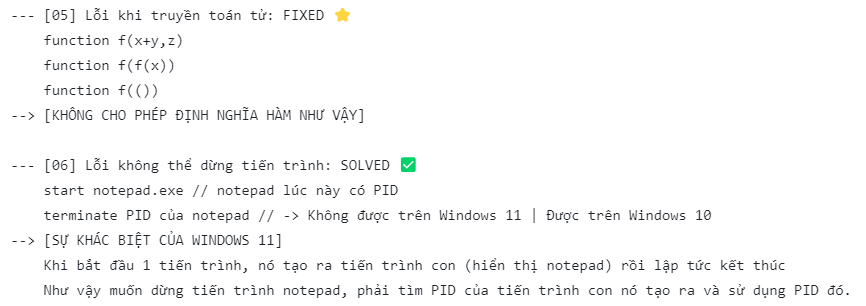
\includegraphics[width=0.8\textwidth]{images/12.png}
    \caption{Bản ghi lỗi\footnote{\orange{Mã nguồn dự án:} \href{https://github.com/HaiAu2501/Operating-System-Project/blob/main/bug.txt}{Bản ghi lỗi}} và cách khắc phục lỗi}
    \label{fig:enter-label}
\end{figure}
\begin{itemize}
    \item  Áp dụng các nguyên lý \cyan{lập trình hướng đối tượng} trong việc thiết kế và triển khai các tính năng trong Tiny Shell.
    \item Làm việc nhóm hiệu quả, chia sẻ kiến thức và phân công công việc một cách hợp lý.
\end{itemize}
\end{frame}

\subsection{Khó khăn và giải pháp}
\begin{frame}{Khó khăn}
\begin{itemize}
    \item Việc xây dựng bộ phân tích cú pháp để hiểu và xử lý đúng các lệnh từ người dùng gặp nhiều thách thức.\\
    $\to$ Đảm bảo rằng các lệnh sai cú pháp được phát hiện và thông báo lỗi một cách rõ ràng cho người dùng.\\
    $\to$ Xử lý các đường dẫn tệp, bao gồm đường dẫn tương đối và tuyệt đối.\\
    $\to$ Quản lý các tín hiệu hệ thống như SIGINT (Ctrl + C).
    \item Khó khăn khi xử lý các lệnh có cú pháp phức tạp như lệnh điều kiện, vòng lặp, và các biểu thức toán học.
    \item Đối mặt với các lỗi phát sinh, thiếu nhất quán trong tổ chức mã nguồn.
\end{itemize}
\end{frame}

\begin{frame}{Giải pháp}
\begin{itemize}
    \item Thực hiện tối ưu hóa mã nguồn để Tiny Shell hoạt động hiệu quả, không tiêu tốn quá nhiều tài nguyên hệ thống.
    \item Liên tục kiểm thử, tối ưu hóa và sửa lỗi, phát triển các kịch bản kiểm thử với độ khó cao.
    \item Thử thách trước cú pháp và tính năng phức tạp.
\end{itemize}
\end{frame}

\begin{frame}
    \begin{columns}
        \begin{column}{0.45\textwidth}
            \centering
            \Large \orange{Cảm ơn thầy và các bạn đã lắng nghe!}
        \end{column}
        \begin{column}{1 pt}
            \centering
            \textcolor{cyan}{\rule{1pt}{200pt}}
        \end{column}
        \begin{column}{0.45\textwidth}
            \begin{itemize}
                \item \cyan{Email:} tuankiet.nv2501@gmail.com
                \item \cyan{GitHub:} \href{https://github.com/HaiAu2501}{HaiAu2501}
                \item \cyan{Phone:} +84978 621 832
            \end{itemize}
        \end{column}
    \end{columns}
    
\end{frame}

\end{document}
